%%%%%%%%%%%%%%%%%%%%%%%%%%%%%%%%%%%%%%%%%%%%%%%%%%%%%%%%%%%%%%%%%%%%%%%%%%%%%%%%%%%%
%%----------------------------------------------------------------------------------
% DO NOT Change this is the required setting A4 page, 11pt, onside
% print, book style
%%----------------------------------------------------------------------------------
\documentclass[a4paper,11pt,oneside]{book}
\usepackage{CS_report} % DO NOT REMOVE THIS LINE.
%%%%%%%%%%%%%%%%%%%%%%%%%%%%%%%%%%%%%%%%%%%%%%%%%%%%%%%%%%%%%%%%%%%%%%%%%%%%%%%%%%%%

%%%%%%%%%%%%%%%%%%%%%%%%%%%%%%%%%%%%%%%%%%%%%%%%%%%%%%%%%%%%%%%%%%%%%%%%%%%%%%%%%%%%
\begin{document}

\captionsetup[figure]{margin=1.5cm,font=small,name={Figura},labelsep=colon}
\captionsetup[table]{margin=1.5cm,font=small,name={Tabela},labelsep=colon}

\frontmatter

%%%%%%%%%%%%%%%%%%%%%%%%%%%%%%%%%%%%%%%%%%%%%%%%%%%%%%%%%%%%%%%%%%%%%%%%%%%%%%%%
\begin{titlepage}
  \begin{center}
    
\includegraphics[width=3cm]{figures/ufrnlogo.png}\\[0.5cm]
    {\LARGE Universidade Federal do Rio Grande do Norte\\[0.5cm]
    Departamento de Informática e Matemática Aplicada}\\[2cm]

    \linespread{1.2}\huge {
      Relatório da $1^a$ Unidade - Grafos

    }
    \linespread{1}~\\[2cm]
    % {\color{blue} \rule{\textwidth}{1pt}}
    {\Large
      Alexandre Dantas, Andriel Vinicius, Gabriel Carvalho, Maria Paz
      e Vinicius de Lima
    }\\[1cm]

    {\large \emph{Professor:} Matheus Menezes}\\[1cm]

    {\Large \today}
  \end{center}
\end{titlepage}

% -------------------------------------------------------------------
% Contents, list of figures, list of tables
% -------------------------------------------------------------------

\tableofcontents
\listoffigures
\listoftables

%%%%%%%%%%%%%%%%%%%%%%%%%%%%%%%%%%%%%%%%%%%%%%%%%%%%%%%%%%%%%%%%%%%%%%%%
%%                                                                    %%
%%  Main chapters and sections of your project                        %%
%%  Everything from here on needs updates in your own words and works %%
%%                                                                    %%
%%%%%%%%%%%%%%%%%%%%%%%%%%%%%%%%%%%%%%%%%%%%%%%%%%%%%%%%%%%%%%%%%%%%%%%%
\mainmatter
% Read for preparation of document in LaTex
% Lamport, L. (1986), LATEX: A Document Preparation System, Addison-Wesley.

\chapter{Introdução}
\label{ch:intro}

%TODO: Melhorar e extender a introdução
% Isso ficou com uma cara de abstract mal feito...
Este projeto tem como objetivo implementar uma API de
algoritmos relacionados a Grafos na linguagem de programação Rust. A
especificação da API segue as funcionalidades descritas na
definição da Avaliação 01 da disciplina de Grafos, sob o Departamento
de Informática Aplicada (DIMAp) da Universidade Federal do Rio Grande
do Norte (UFRN).

Nesta implementação, a especificação da API se materializa em grande
parte como \emph{traços} (\textit{traits}) de Rust, esse conceito é
semelhante a noção de \textit{interface} em linguagens como Java
e Go e praticamente idêntico ao conceito de \textit{typeclasses} em
linguagens como Haskell, o uso de traços permite que a API seja
flexível e mantenha fidelidade as definições algébricas, além do
mais, permite, por meio da implementação a nível de traço, que o código
seja genérico e eficiente para as diversas representações de grafos.

Além dos traços, fizemos grande uso do conceito de \textit{iteradores}, que
também surgem a partir de traços, essa abstração permite que o código
fique ainda mais reutilizável, sem que a eficiência seja comprometida.

Neste relatório vamos discutir a implementação e apresentar essas
vantagens em detalhes, além disso, vamos demonstrar empiricamente a
partir de testes de benchmark que apesar do alto nível de abstração,
a eficiência dos algoritmos ainda fica a par de implementações ótimas
feitas em C++.

Para assegurar o comportamento esperado dos algoritmos, também
implementamos mais de 50 testes unitários que testam as
validam as implementações. Entretanto, por causa da extensão dos testes, vamos
disponibilizá-los apenas através do código fonte da API.

\section{Especificação da API}
\label{sec:api_spec}

De acordo com a definição da Avaliação 01 a API deve possuir as
seguintes funcionalidades:

\subsection{Para Grafos Não Direcionados}

\begin{enumerate}
  \item Criação do Grafo a partir da Lista de Adjacências.
  \item Criação do Grafo a partir da Matriz de Adjacências.
  \item Criação do Grafo a partir da Matriz de Incidência.
  \item Conversão de matriz de adjacência para lista de Adjacências e
    vice-versa.
  \item Função que calcula o grau de cada vértice.
  \item Função que determina se dois vértices são adjacentes.
  \item Função que determina o número total de vértices.
  \item Função que determina o número total de arestas.
  \item Inclusão de um novo vértice usando Lista de Adjacências e
    Matriz de Adjacências.
  \item Exclusão de um vértice existente usando Lista de Adjacências
    e Matriz de Adjacências.
  \item Função que determina se um grafo é conexo ou não.
  \item Determinar se um grafo é bipartido.
  \item \label{item:bfs1} Busca em Largura, a partir de um vértice específico.
  \item \label{item:dfs1} Busca em Profundidade, com determinação de arestas de
    retorno, a partir de um vértice em específico.
  \item \label{item:biconnect} Determinação de articulações e
    componentes biconexos, utilizando obrigatoriamente a função \texttt{lowpt}.
\end{enumerate}

\subsection{Para Grafos Direcionados (ou Dígrafos)}

\begin{enumerate}[resume]
  \item Representação do Dígrafo a partir da Matriz de Adjacências.
  \item Representação do Dígrafo a partir da Matriz de Incidência.
  \item Determinação do Grafo subjacente.
  \item \label{item:bfs2} Busca em largura.
  \item \label{item:dfs2} Busca em profundidade, com determinação de
    profundidade de entrada de saída de cada vértice, e arestas de
    árvore, retorno, avanço e cruzamento.
\end{enumerate}

\section{Solução proposta}

\subsection{Traços}

Como discutido brevemente no início do capítulo (\ref{ch:intro}),
nossa solução se baseia na criação de traços e iteradores que vão
implementar os algoritmos descritos na especificação da API
(\ref{sec:api_spec}). Em específico, haverá um traço para grafos não
direcionados e um traço para grafo direcionados, onde o traço para
grafos não direcionados herdará as propriedades do traço para grafos
direcionados. Essa abordagem permite que boa parte dos algoritmos
que seriam exclusivos para um tipo de grafo funcione em ambos, a
validade desse design se materializa por meio dos testes unitários
que desenvolvemos para API, que testa diversos casos de uso de cada
implementação para os dois tipos de grafos.

\subsection{Iteradores}

Quanto ao uso de iteradores especificamente, eles serão implementados
para algoritmos que envolvem algum tipo de travessia no grafo, como a
Busca em Profundidade (DFS) nos items~\ref{item:dfs1} e \ref{item:dfs2} e
Busca em Largura (BFS) nos items~\ref{item:bfs1} e \ref{item:bfs2}. A
vantagem de implementar iteradores para esses algoritmos é que a
outros algoritmos como a Determinação de Componentes Biconexos no
item~\ref{item:biconnect} fica derivável da implementação dessas
buscas. Além disso, a implementação em forma de iteradores permite
que possíveis usuários da API tenha acesso ao extenso framework de iteradores
que a biblioteca padrão de Rust oferece. Um exemplo de uso de
iteradores para além da implementação da API, seria a determinação de
ciclos no grafo, determinação de menor caminho entre dois vértices,
busca de um vértice específico, filtragem de vértices durante a
busca, modificação do grafo durante a busca, algoritmos de
backtracking e outros, tudo isso apenas compondo a implementação
inicial com os recursos que o iterador de Rust oferece e sem perder
desempenho em relação a uma implementação tradicional.

% TODO: Refletir sobre se devemos adicionar mais informações sobre a
% solução aqui. Falar mais, por exemplo, de abstrações de custo zero,
% leitura de arquivos, etc.

\section{Organização do relatório}

% TODO: Atualizar referência do capítulo 2.
No capítulo 2, vamos apresentar as definições que vamos usar durante
o relatório e construir a base necessária para que o leitor consiga
acompanhar a parte teórica em sua totalidade. Nessa seção revisaremos conceitos
como definição de grafo, vértices, arestas, adjacência,
conectividade e outros.

% TODO: Atualizar referência do capítulo 3.
No capítulo 3, vamos revisar as representações de grafos nas
estruturas de dados que temos disponíveis na linguagem de
programação, estas são, Lista de Adjacência, Matriz de Adjacência e
Matriz de Incidência. Também vamos discorrer um pouco sobre as
vantagens e desvantagens de cada uma.

% TODO: Atualizar referência do capítulo 4.
No capítulo 4, vamos descrever em uma linguagem de pseudocódigo a
implementação dos algoritmos da especificação da API. Novamente, para
preparar o leitor teoricamente para a implementação em Rust.

% TODO: Atualizar referência do capítulo 5.
No capítulo 5, vamos apresentar e discorrer sobre as partes relevantes
do código em Rust que implementa a API e consequentemente as representações e
algoritmos descritos nos capítulos 3 e 4.

% TODO: Atualizar referência do capítulo 6.
No capítulo 6, vamos demonstrar porque as abstrações utilizadas na
implementação é zero custo comparando sua performance com uma
implementação tradicional em C++.

% TODO: Atualizar referência do capítulo 7.
No capítulo 7, vamos discutir as possíveis melhorias a nossa API e quais
podem ser os futuros próximos passos.

No apêndice A, você poderá consultar as atividades desenvolvidas por
cada integrante.

\chapter{Revisão teórica}
\label{ch:revisão}

As definições utilizadas neste projeto foram, em grande parte,
retiradas de \cite{diestel2025graph}, com algumas modificações. Como
a implementação dos algoritmos está em inglês, também apresentaremos
o correspondente de cada definição em inglês, entre parênteses.

\begin{mydef}[Grafo]
  Um \emph{grafo} (\textit{graph}) é uma estrutura $G := (V, A)$
  tal que $A \subseteq V^2$ e $V$ é um conjunto de um tipo qualquer.
  Os elementos de $V$ são denominados vértices (\textit{nodes}) e os
  elementos de $A$ são denominados de arestas
  (\textit{edges}). O jeito tradicional de visualizar um
  grafo é como uma figura composta de bolas e setas:
  \begin{figure}[h]
    \centering
    \begin{tikzpicture}
      \GraphInit[vstyle=normal]
      \tikzset{EdgeStyle/.style={->}}
      \Vertices{circle}{1,2,3,4}
      \Edges(1,2,3)
      \Edge(1)(4)
    \end{tikzpicture}
    \caption{Um grafo com $V := \{1,2,3,4\}$ e $A :=
    \{(1,2),(1,4),(2,3)\}.$}
    \label{fig:graph1}
  \end{figure}
  \FloatBarrier
\end{mydef}

\begin{mydef}[Ordem e Tamanho]
  O número de vértices de um grafo $G$ é chamado de \emph{ordem}
  (\textit{order}) e é denotado por $|G|$ -- o número de arestas é chamado de
  \emph{tamanho} (\textit{size}) e é denotado por $||G||$. Por exemplo, na
  Figura~\ref{fig:graph1}, $|G| = 4$ e $||G|| = 3$.
\end{mydef}

\begin{mydef}[Adjacência]
  Dizemos que um vértice $v$ é \emph{adjacente}, ou \emph{vizinho},
  de um vértice
  $u$ (\textit{neighbor}) se somente se $(u,v) \in A$, também,
  denotaremos $(u,v)$ como $uv$. Visualmente,
  enxergamos isso como:
  \begin{figure}[h]
    \centering
    \begin{tikzpicture}
      \GraphInit[vstyle=normal]
      \tikzset{EdgeStyle/.style={->}}
      \Vertices{circle}{v,u}
      \Edge(u)(v)
    \end{tikzpicture}
    \caption{Um grafo com $V := \{u,v\}$ e $A :=
    \{(u,v)\}.$}
  \end{figure}
  \FloatBarrier
\end{mydef}

\begin{mydef}[Conjunto de adjacentes]
  Num grafo $G$, o conjunto de todos os vértices adjacentes de $u$
  (\textit{neighbors}) é denotado por $A_G(u) := \{v \in V\, |\, uv \in
  A\}$. Já o conjunto de todos os vértices que em que $v$ é adjacente
  será denotado por $\bar{A}_G(u) := \{ v \in V\, |\, vu \in A\}$.
\end{mydef}

\begin{mydef}[Grau de um vértice]
  O \emph{grau de um vértice} $v$ (\textit{node degree}) é o valor
  correspondente da soma $|A_G(v)| + |\bar{A}_G(v)|$. Também
  denotamos $|A_G(v)|$ como $d^+(v)$, $|\bar{A}_G(v)|$ como $d^-(v)$ e
  sua soma como $d(v)$.
\end{mydef}

\begin{mydef}[Caminho]
  Um \emph{caminho} (\textit{path}) é um grafo $C := (V, A)$ que tem a forma:
  \begin{displaymath}
    V := \{x_0, x_1,...,x_k\} \qquad A := \{x_0x_1,x_1x_2,...,x_{k-1}x_k\}
  \end{displaymath}
  Dizemos que $C$ é um caminho de $x_0$ a $x_k$. Normalmente nos
  referimos ao caminho como a sequência dos seus vértices, $x_0x_1...x_k$.
\end{mydef}

\begin{mydef}[Conectividade]
  Dizemos que um grafo $G$ é conexo (\textit{connected}) se somente
  se para quaisquer dois vértices $u$ e $v$, existe um caminho entre eles.
\end{mydef}

\begin{mydef}[Grafo não direcionado]
  Dizemos que um grafo $G$ é \emph{não direcionado}
  (\textit{undirected}) se somente se $A$ é simétrico, ou seja, se
  $uv \in A$ então $vu \in A$. O nome não direcionado vem da ideia de
  que os grafos que viemos discutindo até agora são denomidados de
  \emph{direcionados}, ou simplesmente \emph{dígrafos}. Na
  literatura é comum apresentar grafo não direcionado como grafo e
  depois o direcionado como dígrafo, resolvemos inverter a ordem pois
  assim se traduz melhor nas representações de grafos que vamos
  implementar. Um grafo não direcionado pode ser visualizado sem a
  ponta das setas:

  \begin{figure}[h]
    \centering
    \begin{tikzpicture}
      \GraphInit[vstyle=normal]
      \Vertices{circle}{c,b,a}
      \Edges(a,b,c)
    \end{tikzpicture}
    \caption{Um grafo não direcionado com $V := \{a,b,c\}$ e $A :=
    \{ab,ba,bc,cb\}$}
    \label{fig:ungraph1}
  \end{figure}

  Também é comum omitir a simetria das arestas se pelo contexto for
  claro que está sendo tratado de um grafo não direcionado, na
  Figura~\ref{fig:ungraph1}, o conjunto de arestas $A$ seria escrito
  como $\{ab,bc\}$.
\end{mydef}

\begin{mydef}[Grafo subjacente]
  O grafo subjacente (\textit{underlying}) de um grafo direcionado $G
  := (V, A)$ é o grafo $S := (V, A')$ onde $A' := \{vu\, |\, uv \in A\} \cup A$.
\end{mydef}

\begin{mydef}[Grafo Bipartido]
  Dizemos que um grafo $G := (V, A)$ é bipartido (\textit{bipartite})
  se somente se existem dois conjuntos disjuntos $V_1$, $V_2$ tal que
  $V_1 \cup V_2 = V$, e que para todo $(u, v) \in A$, ($u \in
  V_1$ e $v \in V_2$) ou ($u \in V_2$ e $v \in V_1$), isto é, toda
  aresta em $A$ conecta um vértice de $V_1$ a um vértice de $V_2$.
  \begin{figure}[h]
    \centering
    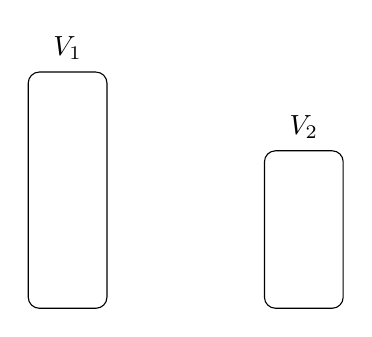
\begin{tikzpicture}
      \GraphInit[vstyle=normal]
      \SetGraphUnit{2}

      % V_1
      \Vertex[x=0,y=3]{a}
      \Vertex[x=0,y=2]{b}
      \Vertex[x=0,y=1]{c}

      % V_2
      \Vertex[x=3,y=2]{u}
      \Vertex[x=3,y=1]{v}

      % Bipartite edges
      \Edge(a)(u)
      \Edge(b)(v)
      \Edge(b)(u)
      \Edge(c)(v)

      % Partitions
      \draw[rounded corners] (-0.5, 0.5) rectangle (0.5, 3.5);
      \node at (0, 3.8) {$V_1$};
      \draw[rounded corners] (2.5, 0.5) rectangle (3.5, 2.5);
      \node at (3, 2.8) {$V_2$};
    \end{tikzpicture}
    \caption{Um grafo bipartido com $V_1 := \{a,b,c\}$ e $V_2 := \{u,v\}$}
  \end{figure}
  \FloatBarrier
\end{mydef}

\begin{mydef}[Grafo Biconexo]
  Dizemos que um grafo $G := (V, A)$ é biconexo
  (\textit{biconnected}) se somente se $|G| > 2$ e para todo $v \in
  V$,  o subgrafo de $G$ resultante da remoção de $v$ é conexo, isto
  é, $G - \{v\}$ é conexo.
\end{mydef}
 %
% replace all text with your own text.
% in this template few examples are mention
\chapter{Methodology}
\label{ch:method} % Label for method chapter

We mentioned in Chapter~\ref{ch:into} %[example backward reference to a chapter or section.]
that a project report's structure could follow a particular paradigm. Hence, the organization of a report (effectively the Table of Content of a report) can vary depending on the type of project you are doing. Check which of the given examples suit your project. Alternatively, follow your supervisor's advice.

\section{Examples of the sections of a methodology chapter}
A general report structure is summarised (suggested) in Table~\ref{tab:gen_template}. Table~\ref{tab:gen_template} describes that, in general, a typical report structure has three main parts: (1) front matter, (2) main text, and (3) end matter. %[\textbf{also notice that the preceding sentence is an example of a numbered list in a text body}]. 
The structure of the front matter and end matter will remain the same for all the undergraduate final year project report. However, the main text varies as per the project's needs.
\begin{table}[!ht]
    \centering
    \caption{Undergraduate report template structure}
    \label{tab:gen_template}
    \begin{tabular}{llll}     
        \toprule
        \multirow{7}{3cm}{Frontmatter} 
        & & Title Page & \\                  
        & & Abstract &    \\          
        & & Acknowledgements & \\                            
        & & Table of Contents &    \\                                
        & & List of Figures   &    \\                        
        & & List of Tables    &    \\                
        & & List of Abbreviations  &    \\                     
        & &   &    \\                        
        \multirow{7}{3cm}{Main text}
        & Chapter 1 & Introduction   &    \\                         
        & Chapter 2 & Literature Review   &    \\
        & Chapter 3 & Methodology   &    \\
        & Chapter 4 & Results    &    \\
        & Chapter 5 & Discussion and Analysis  &    \\
        & Chapter 6 & Conclusions and Future Work  &    \\        
        & Chapter 7 & Refection  &    \\          
        & &   &    \\                       
        \multirow{2}{3cm}{End matter}
        & & References  &    \\   
        & & Appendices (Optional)  &    \\ 
        & & Index (Optional)  &    \\ 
        \bottomrule
    \end{tabular}
\end{table}

\subsection{Example of a software/Web development main text structure}
\label{subsec:se_chpters}
Notice that the ``methodology'' Chapter of Software/Web development in Table~\ref{tab:soft_eng_temp} takes a standard software engineering paradigm (approach). Alternatively, these suggested sections can be the chapters of their own. Also, notice that ``Chapter 5'' in Table~\ref{tab:soft_eng_temp} is ``Testing and Validation'' which is different from the general report template mentioned in Table~\ref{tab:gen_template}. Check with your supervisor if in doubt.
\begin{table}[!ht]
    \centering
    \caption{Example of a software engineering-type report structure}
    \label{tab:soft_eng_temp}
    \begin{tabular}{lll}     
        \toprule                   
        Chapter 1 & Introduction   &    \\        
        Chapter 2 & Literature Review  &    \\                   
        Chapter 3 & Methodology   &    \\
        &               & Requirements specifications   \\
        &               & Analysis   \\
        &               & Design   \\
        &               & Implementations   \\
        Chapter 4 & Testing and Validation  &    \\
        Chapter 5 & Results and Discussion      &    \\
        Chapter 6 & Conclusions and Future Work  &    \\        
        Chapter 7 & Reflection  &    \\                          
        \bottomrule
    \end{tabular}
\end{table}

\subsection{Example of an algorithm analysis main text structure}
Some project might involve the implementation of a state-of-the-art algorithm and its performance analysis and comparison with other algorithms. In that case, the suggestion in Table~\ref{tab:algo_temp} may suit you the best. 
\begin{table}[!ht]
    \centering
    \caption{Example of an algorithm analysis type report structure}
    \label{tab:algo_temp}
    \begin{tabular}{lll}     
        \toprule                   
        Chapter 1 & Introduction  &    \\        
        Chapter 2 & Literature Review  &    \\                
        Chapter 3 & Methodology   &    \\
        &               & Algorithms descriptions  \\
        &               & Implementations   \\
        &               & Experiments design   \\
        Chapter 4 & Results       &  \\
        Chapter 5 & Discussion and Analysis  &    \\
        Chapter 6 & Conclusion and Future Work  &    \\        
        Chapter 7 & Reflection  &    \\          
        \bottomrule
    \end{tabular}
\end{table}

\subsection{Example of an application type main text structure}
If you are applying some algorithms/tools/technologies on some problems/datasets/etc., you may use the methodology section prescribed in Table~\ref{tab:app_temp}.  
\begin{table}[!ht]
    \centering
    \caption{Example of an application type report structure}
    \label{tab:app_temp}
    \begin{tabular}{lll}     
        \toprule                   
        Chapter 1 & Introduction  &    \\        
        Chapter 2 & Literature Review  &    \\                
        Chapter 3 & Methodology   &    \\
        &               & Problems (tasks) descriptions  \\
        &               & Algorithms/tools/technologies/etc. descriptions  \\        
        &               & Implementations   \\
        &               & Experiments design and setup   \\
        Chapter 4 & Results       &  \\
        Chapter 5 & Discussion and Analysis  &    \\
        Chapter 6 & Conclusion and Future Work  &    \\        
        Chapter 7 & Reflection  &    \\          
        \bottomrule
    \end{tabular}
\end{table}

\subsection{Example of a science lab-type main text structure}
If you are doing a science lab experiment type of project, you may use the  methodology section suggested in Table~\ref{tab:lab_temp}. In this kind of project, you may refer to the ``Methodology'' section as ``Materials and Methods.''
\begin{table}[!ht]
    \centering
    \caption{Example of a science lab experiment-type report structure}
    \label{tab:lab_temp}
    \begin{tabular}{lll}     
        \toprule                   
        Chapter 1 & Introduction  &    \\        
        Chapter 2 & Literature Review  &    \\                
        Chapter 3 & Materials and Methods   &    \\
        &               & Problems (tasks) description  \\
        &               & Materials \\        
        &               & Procedures  \\                
        &               & Implementations   \\
        &               & Experiment set-up   \\
        Chapter 4 & Results       &  \\
        Chapter 5 & Discussion and Analysis  &    \\
        Chapter 6 & Conclusion and Future Work  &    \\        
        Chapter 7 & Reflection  &    \\          
        \bottomrule
    \end{tabular}
\end{table}

\subsection{Ethical considerations}
This section addresses ethical aspects of your project. This may include:
    informed consent, describing how participants will be informed about the study's purpose, procedures, risks, and benefits. You should detail the process used for obtaining consent and ensuring participants understand their rights.


\begin{itemize}
    \item \textbf{Informed Consent}: If data was collected from participant, detail the process for obtaining consent and ensuring participants understand their rights.
    
    \item \textbf{Confidentiality and Privacy}: Explain measures taken to protect participants' data and maintain confidentiality. Discuss how data is stored, who will have access, and how anonymity will be preserved.
    
    \item \textbf{Risk Assessment}: Identify potential risks to participants and outline strategies to minimize them. 
    
    \item \textbf{Vulnerable Populations}: If applicable, address how you will protect vulnerable groups (e.g., children, elderly, or marginalized communities) involved in your project. 
    
    \item \textbf{Research Integrity}: Highlight your commitment to honesty and transparency in research. Discuss how you will avoid plagiarism, fabrication, and falsification of data.
    
    \item \textbf{Compliance with Regulations}: Mention relevant ethical guidelines and regulations that your project will adhere to.
    
    \item \textbf{Impact on Society}: Reflect on the broader implications of your project. Discuss how the outcomes may affect communities, stakeholders, or the environment, and how you plan to address any potential negative consequences.
    
    \item \textbf{Feedback Mechanisms}: Describe how you incorporate feedback from participants and stakeholders to improve the ethical conduct of the project throughout its duration.

\end{itemize}


\section{Example of an Equation in \LaTeX}
Eq.~\ref{eq:eq_example} [note that this is an example of an equation's in-text citation] is an example of an equation in \LaTeX. In Eq.~\eqref{eq:eq_example}, $ s $ is the mean of elements $ x_i \in \mathbf{x} $: 

\begin{equation}
\label{eq:eq_example} % label used to refer the eq in text
s = \frac{1}{N} \sum_{i = 1}^{N} x_i. 
\end{equation}

Have you noticed that all the variables of the equation are defined using the \textbf{in-text} maths command \$.\$, and Eq.~\eqref{eq:eq_example} is treated as a part of the sentence with proper punctuation? Always treat an equation or expression as a part of the sentence. 



\section{Example of a Figure in \LaTeX}
Figure~\ref{fig:chart_a} is an example of a figure in \LaTeX. For more details, check the link:

\href{https://en.wikibooks.org/wiki/LaTeX/Floats,_Figures_and_Captions}{wikibooks.org/wiki/LaTeX/Floats,\_Figures\_and\_Captions}.

\noindent
Keep your artwork (graphics, figures, illustrations) clean and readable. At least 300dpi is a good resolution of a PNG format artwork. However, an SVG format artwork saved as a PDF will produce the best quality graphics. There are numerous tools out there that can produce vector graphics and let you save that as an SVG file and/or as a PDF file. One example of such a tool is the ``Flow algorithm software''. Here is the link for that: \href{http://www.flowgorithm.org/download/}{flowgorithm.org}.
\begin{figure}[!ht]
    \centering
    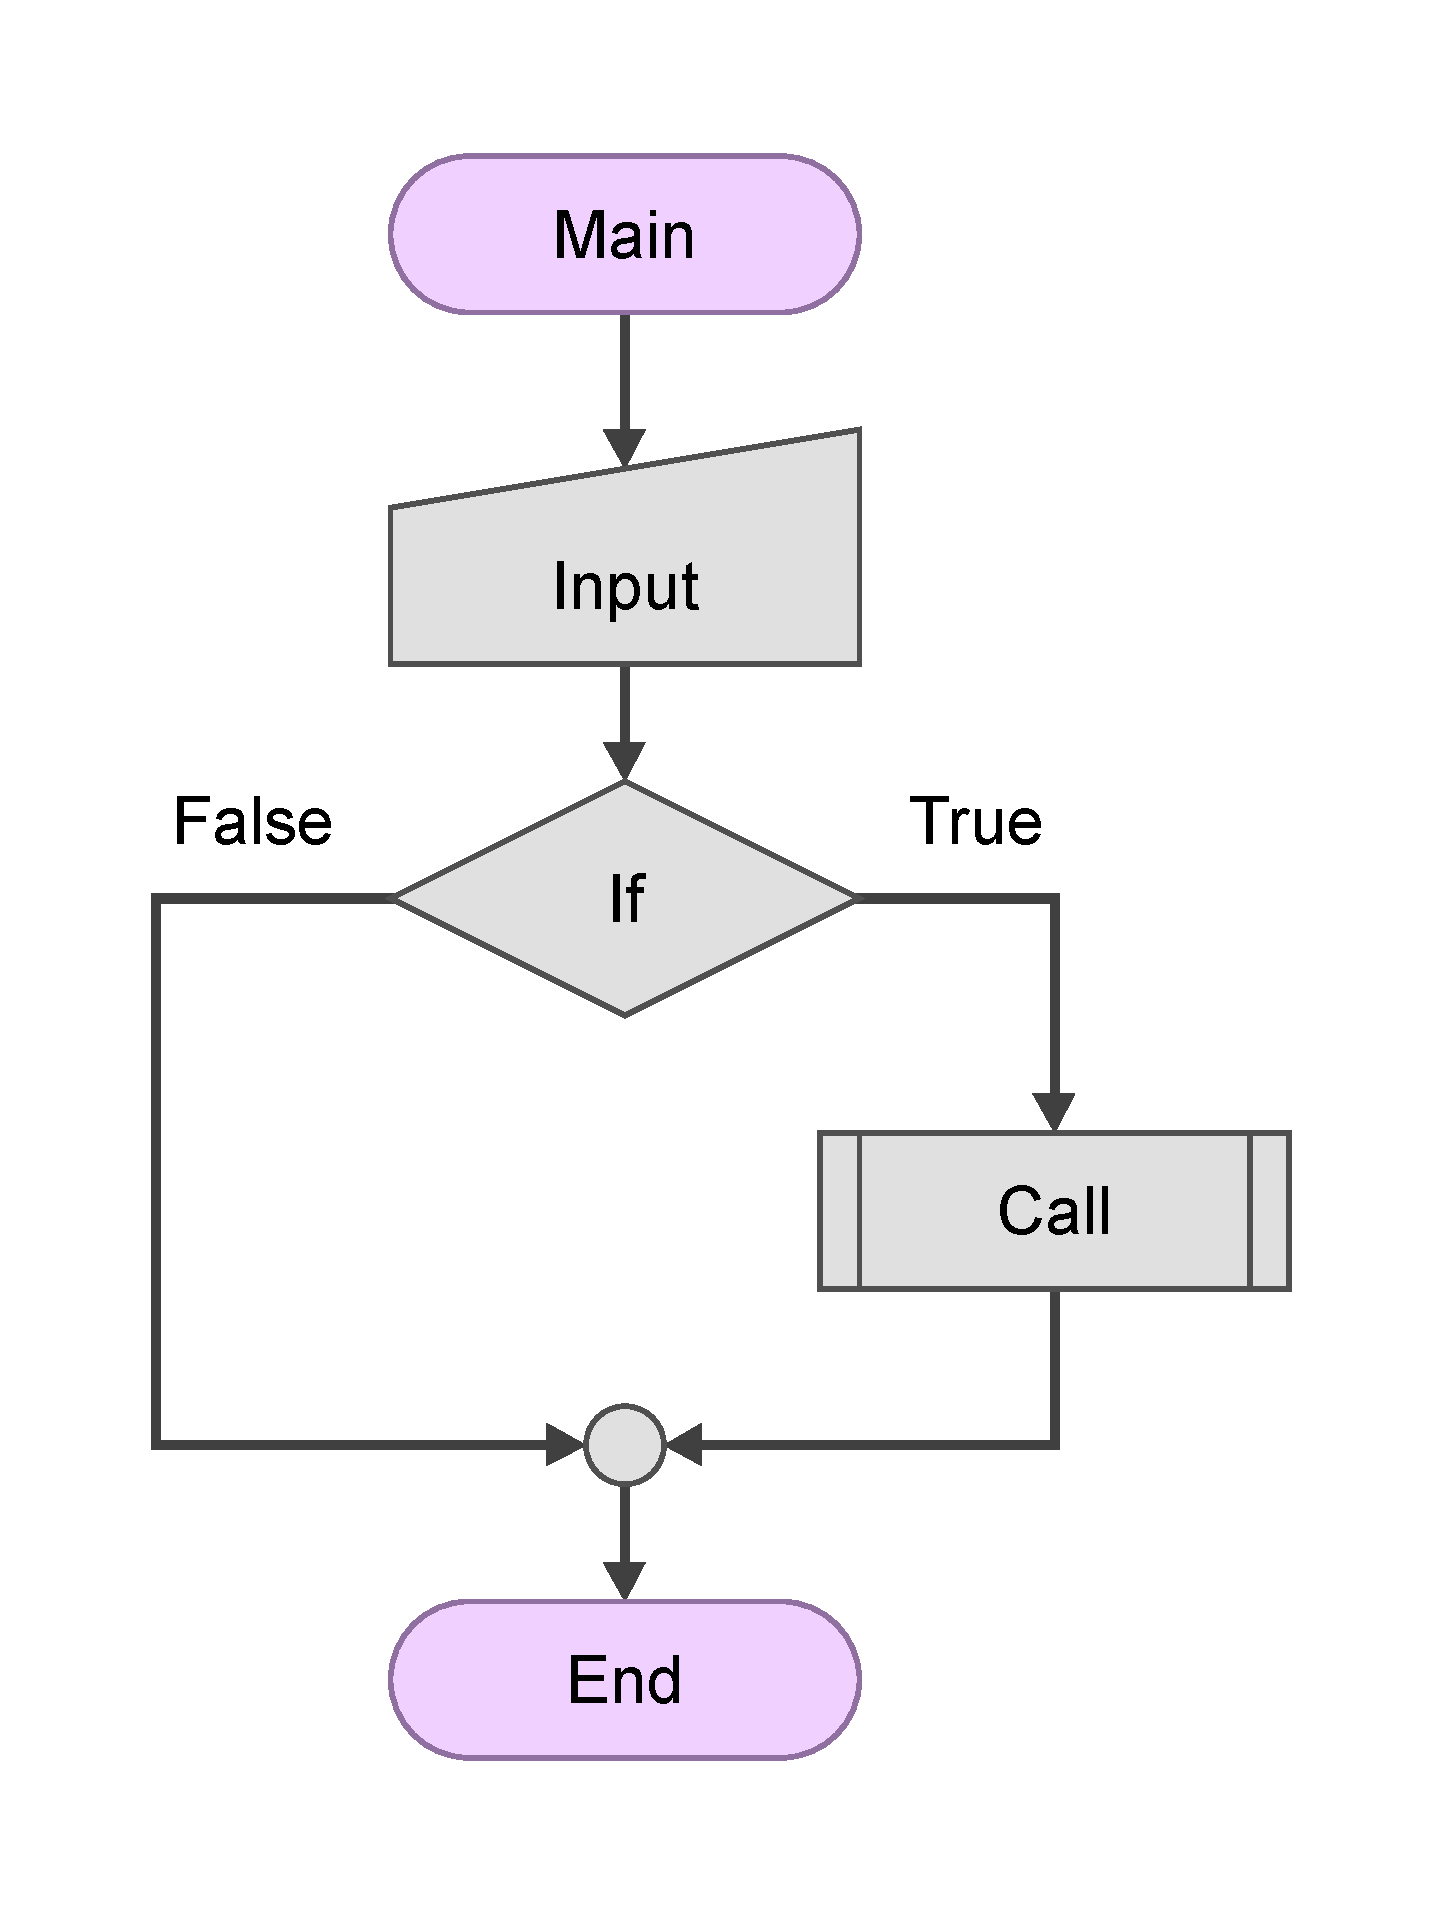
\includegraphics[scale=0.3]{figures/chart.pdf}
    \caption{Example figure in \LaTeX.}
    \label{fig:chart_a}
\end{figure}

\clearpage %  use command \clearpage when you want section or text to appear in the next page.

\section{Example of an algorithm in \LaTeX}
Algorithm~\ref{algo:algo_example} is a good example of an algorithm in \LaTeX.  
\begin{algorithm}
    \caption{Example caption: sum of all even numbers}
    \label{algo:algo_example}
    \begin{algorithmic}[1]
        \Require{$ \mathbf{x}  = x_1, x_2, \ldots, x_N$}
        \Ensure{$EvenSum$ (Sum of even numbers in $ \mathbf{x} $)}
        \Statex
        \Function{EvenSummation}{$\mathbf{x}$}
        \State {$EvenSum$ $\gets$ {$0$}}
        \State {$N$ $\gets$ {$length(\mathbf{x})$}}
        \For{$i \gets 1$ to $N$}                    
        \If{$ x_i\mod 2 == 0$}  \Comment Check whether a number is even.
        \State {$EvenSum$ $\gets$ {$EvenSum + x_i$}}
        \EndIf
        \EndFor
        \State \Return {$EvenSum$}
        \EndFunction
    \end{algorithmic}
\end{algorithm}
 
\section{Example of code snippet  in \LaTeX}

Code Listing~\ref{list:python_code_ex} is a good example of including a code snippet in a report. While using code snippets, take care of the following:
\begin{itemize}
    \item do not paste your entire code (implementation) or everything you have coded. Add code snippets only. 
    \item The algorithm shown in Algorithm~\ref{algo:algo_example} is usually preferred over code snippets in a technical/scientific report. 
    \item Make sure the entire code snippet or algorithm stays on a single page and does not overflow to another page(s).  
\end{itemize}

Here are three examples of code snippets for three different languages (Python, Java, and CPP) illustrated in Listings~\ref{list:python_code_ex}, \ref{list:java_code_ex}, and \ref{list:cpp_code_ex} respectively.  

\begin{lstlisting}[language=Python, caption={Code snippet in \LaTeX ~and  this is a Python code example}, label=list:python_code_ex]
import numpy as np

x  = [0, 1, 2, 3, 4, 5] # assign values to an array
evenSum = evenSummation(x) # call a function

def evenSummation(x):
    evenSum = 0
    n = len(x)
    for i in range(n):
        if np.mod(x[i],2) == 0: # check if a number is even?
            evenSum = evenSum + x[i]
    return evenSum
\end{lstlisting}

Here we used  the ``\textbackslash clearpage'' command and forced-out the second listing example onto the next page. 
\clearpage  %
\begin{lstlisting}[language=Java, caption={Code snippet in \LaTeX ~and  this is a Java code example}, label=list:java_code_ex]
public class EvenSum{ 
    public static int evenSummation(int[] x){
        int evenSum = 0;
        int n = x.length;
        for(int i = 0; i < n; i++){
            if(x[i]%2 == 0){ // check if a number is even?
                evenSum = evenSum + x[i];
            }
        }
        return evenSum;     
    }
    public static void main(String[] args){ 
        int[] x  = {0, 1, 2, 3, 4, 5}; // assign values to an array
        int evenSum = evenSummation(x);
        System.out.println(evenSum);
    } 
} 
\end{lstlisting}


\begin{lstlisting}[language=C, caption={Code snippet in \LaTeX ~and  this is a C/C++ code example}, label=list:cpp_code_ex]
int evenSummation(int x[]){
    int evenSum = 0;
    int n = sizeof(x);
    for(int i = 0; i < n; i++){
        if(x[i]%2 == 0){ // check if a number is even?
            evenSum = evenSum + x[i];
    	}
    }
    return evenSum;     
}

int main(){
    int x[]  = {0, 1, 2, 3, 4, 5}; // assign values to an array
    int evenSum = evenSummation(x);
    cout<<evenSum;
    return 0;
}
\end{lstlisting}



\section{Example of in-text citation style}
\subsection{Example of the equations and illustrations placement and reference in the text}
Make sure whenever you refer to the equations, tables, figures, algorithms,  and listings for the first time, they also appear (placed) somewhere on the same page or in the following page(s). Always make sure to refer to the equations, tables and figures used in the report. Do not leave them without an \textbf{in-text citation}. You can refer to equations, tables and figures more them once.

\subsection{Example of the equations and illustrations style}
Write \textbf{Eq.} with an uppercase ``Eq`` for an equation before using an equation number with (\textbackslash eqref\{.\}). Use ``Table'' to refer to a table, ``Figure'' to refer to a figure, ``Algorithm'' to refer to an algorithm and ``Listing'' to refer to listings (code snippets). Note that, we do not use the articles ``a,'' ``an,'' and ``the'' before the words Eq., Figure, Table, and Listing, but you may use an article for referring the words figure, table, etc. in general.

For example, the sentence ``A report structure is shown in \textbf{the} Table~\ref{tab:gen_template}'' should be written as ``A report structure is shown \textbf{in} Table~\ref{tab:gen_template}.'' 

\subsection{Tools for In-text Referencing}\label{subsec:reftools}
You will have noticed that there are linked references within the text to specific items in this document (e.g., equations, figures, tables, chapters, sections, etc.).  This is enabled by a combination of \verb|\label{}| and \verb|\ref{}| commands.  The former is typically ``attached'' to an object/section to be labeled, for instance: \lstinline!\section{My Section}\label{sec:my}!.  This label, \verb|sec:my|, can then be used to create an in-text reference (with link) to the referenced object: \verb|\ref{sec:my}|.

The in-text references to the preceding equation were written as: \lstinline!Eq.~\eqref{eq:eq_example}!.  Here, the author needed to explicitly write the \verb|Eq.| text, include a tilde, \verb|~|, to ensure that the text is not separated from the number at a line break, and used \verb|eqref| to automate placement of parentheses around the number.  Alternatively, we could use the cleverref system to reference this item with \verb|\Cref{eq:eq_example}|, yielding: \Cref{eq:eq_example}.  This makes the textual part (Equation) automatic along with spacing and other formatting.  The capital \verb|C| in that command specifies capitalisation of the word, whereas lowercase for a figure item would, \verb|\cref{fig:chart_a}| would yield a lowercase abbreviated form: \cref{fig:chart_a}.

\section{Summary}
Write a summary of this chapter.

~\\[5em]
\noindent
{\huge\textbf{Note:}} In the case of \textbf{software engineering} project a Chapter ``\textbf{Testing and Validation}'' should precede the ``Results'' chapter. See Section~\ref{subsec:se_chpters} for report organization of such project. 


\chapter{Descrição em Pseudocódigo dos Algoritmos da API}
\label{ch:pseudocode}

Neste capítulo, apresentamos a descrição, em linguagem de pseudocódigo, dos principais algoritmos definidos na especificação da API. O objetivo é proporcionar uma visão clara do funcionamento lógico das rotinas antes de sua implementação em Rust, estabelecendo um elo entre o modelo conceitual e o código-fonte.

Cada algoritmo é expresso de forma estruturada e independente de linguagem, destacando apenas o fluxo essencial das operações. Essa abordagem facilita a compreensão dos procedimentos, sem se prender a detalhes sintáticos da linguagem de implementação.

\section{Dígrafos}
O \texttt{trait} \texttt{Graph} é responsável por explicitar qual assinatura as funções que devem ser implementadas. Tal abordagem é coerente pois, como grafo se trata de um Tipo Abstrato de Dado, a implementação é uma particularização de cada Estrutura de Dados. E dentre a funções solicitadas para que uma estrutura possa implementar o trait grafo temos:

\begin{itemize}
  \item Criar um grafo vazio
  \item Ordem e tamanho do grafo
  \item Nós do grafo(através de um iterador)
  \item Adicionar vértices e arestas
  \item Remover nós e arestas
  \item Vizinhos de um nós(através de um iterador)
  \item Determinar se o grafo é bipartido
  \item Grafo subjacente
  \item Se dois nós compartilham uma aresta
  \item Grau de um nó
  \item Iterador a partir de uma BFS
  \item Iterador a partir de uma DFS
  \item Classificar arestas
\end{itemize}

\section{Grafos Não Direcionados}

O \texttt{trait} \texttt{UndirectedGraph} estende o conceito de \texttt{Graph}, representando grafos em que as arestas não possuem direção. E uma vez que só se pode implementar caso \texttt{Graph} já tenha sido implementado anteriormente, a implementação das novas funções é trivial na maioria dos casos, pois recorre às implementações de \texttt{Graph}. A API define métodos específicos para:

\begin{itemize}
    \item Adicionar vértices e arestas;
    \item Remover vértices e arestas;
    \item Obter vizinhos de um vértice;
    \item Determinar se o grafo é conexo
    \item Grau de um nó
    \item Iterador a partir de uma BFS
    \item Iterador a partir de uma DFS
    \item Identificar componentes biconexas(através de um iterador)
\end{itemize}

Grafos não direcionados são fundamentais para modelar problemas onde a direção não é relevante.

\section{Descrição em Pseudocódigo dos Algoritmos}

A seguir, apresentamos os algoritmos da API em pseudocódigo. O objetivo é destacar sua lógica fundamental, sem referência direta à sintaxe de Rust, mas mantendo correspondência com o comportamento esperado dos iteradores.

\subsection{Busca em Profundidade (DFS)}

A busca em profundidade percorre o grafo a partir de um vértice inicial, explorando recursivamente os caminhos até o limite de cada ramo. 

\begin{algorithm}
  \caption{Busca em Profundidade}
  \label{algo:algo_example}
  \begin{algorithmic}[0]
    \Require{$ \mathbf{G(V,A)}$, $v \in \mathbf{V}$}
    \Ensure{$predecessor$ = [ ] (Lista do vizinho de cada vértice)}
    \Statex
    \Function{DFS}{$\mathbf{G(V,A), v}$}
    \State {$predecessor$ $\gets$ [ ]}
    \State {$predecessor[v]$ $\gets$ nulo}
    \Statex
    \State {$visitado$ $\gets$ [ ]}
    \State {$visitado[v]$ $\gets$ $\mathbf{1}$}
    \Statex
    \State {$pilha$ $\gets$ [ ]}
    \State {$pilha$ $\gets$ $empilhar(\mathbf{v})$}
    \Statex
    \While{pilha.tamanho() > 0}
    \State {$u$ $\gets$ $topo(\mathbf{pilha})$}
    \If{$ \exists$ uw $\in A(G)$ $\textbf{e}$ $visitado[w] \neq 1$}
    \State {$predecessor[w]$ $\gets$ $\mathbf{u}$}
    \State {$visitado[w]$ $\gets$ $\mathbf{1}$}
    \State {$pilha$ $\gets$ {$empilhar(\textbf{w})$}}
    \Else
    \State {$pilha$ $\gets$ $desempilhar()$}
    \EndIf
    \EndWhile
    \State \Return {$predecessor$}
    \EndFunction
  \end{algorithmic}
\end{algorithm}

Essa lógica permite identificar ciclos, classificar arestas e analisar conectividade de forma eficiente.

\subsection{Busca em Largura (BFS)}

A busca em largura percorre o grafo por camadas, processando primeiro todos os vértices a uma mesma distância do ponto inicial antes de avançar para os níveis seguintes. O pseudocódigo é apresentado abaixo:

\begin{algorithm}
  \caption{Busca em Largura}
  \label{algo:algo_example}
  \begin{algorithmic}[1]
    \Require{$ \mathbf{G(V,A)}$, $v \in \mathbf{V}$}
    \Ensure{$predecessor$ = [ ] (Lista do vizinho de cada vértice)}
    \Statex
    \Function{BFS}{$\mathbf{G(V,A), v}$}
    \State {$predecessor$ $\gets$ [ ]}
    \State {$predecessor[v]$ $\gets$ nulo}
    \Statex
    \State {$visitado$ $\gets$ [ ]}
    \State {$visitado[v]$ $\gets$ $\mathbf{1}$}
    \Statex
    \State {$fila$ $\gets$ [ ]}
    \State {$fila$ $\gets$ $enfileirar(\mathbf{v})$}
    \Statex
    \While{fila.tamanho() > 0}
    \State {$u$ $\gets$ $começo(\mathbf{fila})$}
    \State {$fila$ $\gets$ $desenfileirar()$}
    \For{$v \in $ u.vizinhos()}
    \If{$visitado[v] \neq 1$}
    \State {$predecessor[v]$ $\gets$ $\mathbf{u}$}
    \State {$visitado[v]$ $\gets$ $\mathbf{1}$}
    \State {$fila$ $\gets$ {$enfileirar(\textbf{v})$}}
    \EndIf
    \EndFor
    \EndWhile
    \State \Return {$predecessor$}
    \EndFunction
  \end{algorithmic}
\end{algorithm}

O BFS é útil em problemas que requerem a descoberta de caminhos mínimos ou a análise de níveis de distância em grafos.

\subsection{Classificação de Arestas}

Durante a DFS, é possível classificar as arestas em diferentes categorias, que auxiliam na análise estrutural do dígrafo:

\begin{itemize}
    \item \textbf{Tree Edge (Árvore):} Conecta um vértice a um filho na DFS.
    \item \textbf{Back Edge (Retorno):} Conecta um vértice a um ancestral, indicando ciclo.
    \item \textbf{Forward Edge (Avanço):} Conecta um vértice a um descendente não filho.
    \item \textbf{Cross Edge (Cruzamento):} Conecta vértices em diferentes ramos da DFS.
\end{itemize}

\subsection{Componentes Biconexas}

O algoritmo permite identificar componentes biconexas em grafos não direcionados. Mantém pilhas de arestas e tempos de descoberta para determinar subconjuntos de vértices que formam componentes biconexas.

\begin{algorithm}
  \caption{Componentes Bicônexas}
  \label{algo:biconnected}
  \begin{algorithmic}[1]
    \Require{$\mathbf{G(V,A)}$}
    \Ensure{Conjunto das componentes bicônexas de $\mathbf{G}$}
    \Statex
    \State {$visitado \gets [\,]$}
    \State {$descoberta \gets [\,]$}
    \State {$baixo \gets [\,]$}
    \State {$pilha \gets [\,]$}
    \State {$componentes \gets [\,]$}
    \State {$tempo \gets 0$}
    \Statex
    \Function{biconnected}{$\mathbf{G(V,A)}$}
      \For{$v \in \mathbf{V}$}
        \If{$visitado[v] \neq 1$}
          \State \Call{dfs\_biconnected}{$\mathbf{G, v, pai = nulo}$}
        \EndIf
      \EndFor
      \State \Return{$componentes$}
    \EndFunction
    \Statex
    \Function{dfs\_biconnected}{$\mathbf{G, v, pai}$}
      \State {$visitado[v] \gets 1$}
      \State {$tempo \gets tempo + 1$}
      \State {$descoberta[v] \gets tempo$}
      \State {$baixo[v] \gets tempo$}
      \Statex
      \For{$u \in v.vizinhos()$}
        \If{$visitado[u] \neq 1$}
          \State {$pilha$ $\gets$ {$empilhar(\textbf{(v,u)})$}}
          \State \Call{dfs\_biconnected}{$\mathbf{G, u, v}$}
          \State {$baixo[v] \gets \min(baixo[v], baixo[u])$}
          \If{$baixo[u] \geq descoberta[v]$}
            \State {$temp \gets [\,]$}
            \While{$pilha.topo() \neq (v, u)$}
              \State {$pilha$ $\gets$ {$desempilhar()$}}
              \State {$temp$ $\gets$ {$adicionar(\textbf{(v',u')})$}}
            \EndWhile
            \State {$componentes$ $\gets$ temp}
          \EndIf
        \ElsIf{$u \neq pai$ \textbf{ e } $descoberta[u] < descoberta[v]$}
          \State {$pilha$ $\gets$ {$empilhar(\textbf{(v,u)})$}}
          \State {$baixo[v] \gets \min(baixo[v], descoberta[u])$}
        \EndIf
      \EndFor
    \EndFunction
  \end{algorithmic}
\end{algorithm}

O algoritmo também permite analisar a conectividade crítica do grafo, identificando vértices e arestas cuja remoção aumentaria o número de componentes conectadas.

No capítulo seguinte os conceitos abordados neste serão implementados para Lista de Adjacência, Matrix de Adjacência e Matriz de Incidência.

\chapter{Implementação}
\label{ch:implementation}

Nesse capítulo serão explicadas as particularidades de cada implementacão das funcões mencionadas no capítulo anterior. Também serão elucidados alguns aspectos exclusivos da linguagem Rust, primeiramente abordando algumas decisões de arquitetura e em seguida falando sobre as 3 estruturas de dados implementadas.

\section{Arquitetura}

Como já citado no capítulos anterior, dado que haveriam implementações de funções em comum para estruturas de dados diferentes, grafo e dígrafo foram implementados através de \texttt{traits}, da seguinte forma:

\begin{lstlisting}[language=Java, caption={Implementação do trait Graph}, label=list:trait_graph]
pub trait Graph<Node: Eq + Hash + Copy> {
    fn new_empty() -> Self;

    fn order(&self) -> usize;

    fn size(&self) -> usize;

    fn node_degrees(&self, n: Node) -> (usize, usize);

    fn nodes(&self) -> impl Iterator<Item = Node>;

    fn add_node(&mut self, n: Node);

    fn remove_node(&mut self, n: Node);

    fn add_edge(&mut self, n: Node, m: Node);

    fn remove_edge(&mut self, n: Node, m: Node);

    type Neighbors<'a>: Iterator<Item = Node>
    where
        Self: 'a,
        Node: 'a;
    fn neighbors<'a>(&'a self, n: Node) -> Self::Neighbors<'a>;

    fn biparted(&self) -> bool;

    fn underlying_graph(&self) -> Self;

    fn has_edge(&self, n: Node, m: Node) -> bool {
        self.neighbors(n).any(|neighbor| neighbor == m)
    }

    fn dfs(&self, start: Node) -> DfsIter<'_, Node, Self>
    where
        Self: Sized,
    {
        DfsIter::new(self, start)
    }

    fn bfs(&self, start: Node) -> BfsIter<'_, Node, Self>
    where
        Self: Sized,
    {
        BfsIter::new(self, start)
    }

    fn classify_edges(&self, start: Node) -> DfsEdgesIter<'_, Node, Self>
    where
        Self: Sized,
    {
        DfsEdgesIter::new(self, start)
    }
}
\end{lstlisting}

As particularidades da sintaxe acima são que, \texttt{Graph} pode ser implementado para qualquer tipo genérico \texttt{N}, desde que este implemente os seguintes \textt{traits}:

\begin{itemize}
  \item \textbf{Eq}: Que dá ao tipo a propriedade de igualdade através do operador ==
  \item \textbf{Hash}: Propriedade necessária para que aquele tipo possa ser usado em estruturas de dados como \texttt{HashMap/HashSet}. Que serão usadas em trabalhos futuros.
  \item \textbf{Copy}: Que dá ao tipo a propriedade de ser copiável através do operador =, o que apesar de parecer trivial, não é. E isso acontece pois Rust introduz o conceito de \cite{ownership}, que faz com que nem todo tipo seja copiável.
\end{itemize}

Feito isso, basta com que o tipo implementa as funções com as assinaturas solicitadas e ele terá o \texttt{trait Graph}. E além dele, também temos outro \texttt{trait} que tem ele como pré-requisito para implementação, o \texttt{UndirectedGraph}:

\begin{lstlisting}[language=Java, caption={Implementação do trait UndirectedGraph}, label=list:trait_undirected_graph]
pub trait UndirectedGraph<Node: Copy + Eq + Hash>: Graph<Node> {
    fn undirected_size(&self) -> usize;

    fn connected(&self) -> bool;

    fn biconnected_components(&self, start: Node) -> BiconnectedComponentsIter<'_, Node, Self>
    where
        Self: Sized,
    {
        BiconnectedComponentsIter::new(self, start)
    }

    fn add_undirected_edge(&mut self, n: Node, m: Node) {
        self.add_edge(n, m);
        self.add_edge(m, n);
    }

    fn remove_undirected_edge(&mut self, n: Node, m: Node) {
        self.remove_edge(n, m);
        self.remove_edge(m, n);
    }

    fn undirected_node_degree(&self, n: Node) -> usize {
        self.neighbors(n).count()
    }

    fn classify_undirected_edges<'a>(&'a self, start: Node) -> impl Iterator<Item = Edge<Node>>
    where
        Self: Sized,
        Node: 'a,
    {
        DfsEdgesIter::new(self, start)
            .filter(|edge| matches!(edge, Edge::Tree(_, _) | Edge::Back(_, _)))
    }
}
\end{lstlisting}

Note que o \texttt{trait} já tem várias implementações, e isso só é possível pois ele usa as funcões já implementadas em \textt{Graph}. Por isso que implementar \textt{UndirectedGraph}, antes, é necessário implementar esse.

Mas feitas as considerações iniciais acerca da arquitetura da implementação, podemos abordar as particularidades de cada Estrutura da Dados.

\section{Matriz de Adjacência}

A Matriz de Adjacência, conforme falado anteriormente, é uma das formas mais comuns de se implementar um grafo. Muito disso em decorrência de sua baixa complexidade na inserção e no acesso nos elementos. Sendo assim, ela é implementada da seguinte forma:

\begin{lstlisting}[language=Java, caption={Implementação da Estrutura de Dados Matriz de Adjacência}, label=list:struct_adj_mat]
#[derive(Debug, Clone)]
pub struct AdjacencyMatrix(pub Vec<Vec<usize>>);
\end{lstlisting}

No código acima, o \texttt{derive} é uma instrução para o compilador inferir como adicionar as pripriedades \texttt{Debug} e \texttt{Clone} na estrutura abaixo. Estrutura essa que consiste em um vetor de vetores de \texttt{usize}(inteiros não-negativos, tipo usado para fins de simplificação, uma vez que temos mais garantias sobre as propridades dele dessa forma, diferente de em tipos genéricos). E abaixo segue a implementação das funções solicitadas pelo \texttt{trait UndirectedGraph}.

\begin{lstlisting}[language=Java, caption={Implementação de UndirectedGraph na Estrutura de Dados Matriz de Adjacência}, label=list:impl_adj_mat_ug] impl UndirectedGraph<usize> for AdjacencyMatrix {
    fn undirected_size(&self) -> usize {
        let mut size = 0;
        for i in 0..self.order() {
            for j in 0..=i {
                if self.0[i][j] > 0 {
                    size += 1;
                }
            }
        }
        size
    }

    fn connected(&self) -> bool {
        let n = self.order();
        if n == 0 {
            return true;
        }

        let mut visited = vec![false; n];
        let mut stack = vec![0];
        visited[0] = true;

        while let Some(u) = stack.pop() {
            for (v, &is_edge) in self.0[u].iter().enumerate() {
                if is_edge > 0 && !visited[v] {
                    visited[v] = true;
                    stack.push(v);
                }
            }
        }

        visited.into_iter().all(|v| v)
    }

    fn undirected_node_degree(&self, node: usize) -> usize {
        if let Some(row) = self.0.get(node) {
            row.iter().filter(|&&val| val != 0).count()
        } else {
            0
        }
    }
}
\end{lstlisting}

Note que ele só define as funções que não tem implementação padrão. E algo que também importante para se pontuar é que a palavra \texttt{mut}(abreviação de "mutável") é requerida sempre que desejamos alterar o valor da variável em questão, pois devemos fazer isso de forma explícita, e isso acontece por conta do conceito de \cite{ownership}. E abaixo segue a implementação de \texttt{Graph}:

\begin{lstlisting}[language=Java, caption={Implementação de Graph na Estrutura de Dados Matriz de Adjacência}, label=list:impl_adj_mat_g]
impl Graph<usize> for AdjacencyMatrix {
    fn new_empty() -> Self {
        AdjacencyMatrix(vec![])
    }

    fn order(&self) -> usize {
        self.0.len()
    }

    fn size(&self) -> usize {
        self.0
            .iter()
            .enumerate()
            .map(|(i, _)| self.neighbors(i).count())
            .sum()
    }

    fn node_degrees(&self, n: usize) -> (usize, usize) {
        let out_deg = self.0[n].iter().filter(|&&v| v != 0).count();
        let in_deg = self.0.iter().filter(|row| row[n] != 0).count();
        (in_deg, out_deg)
    }

    fn nodes(&self) -> impl Iterator<Item = usize> {
        0..self.order()
    }

    fn add_node(&mut self, _n: usize) {
        self.0.push(Vec::new());
        let new_order = self.order();

        for r in &mut self.0 {
            while r.len() < new_order {
                r.push(0);
            }
        }
    }

    fn remove_node(&mut self, n: usize) {
        if n < self.0.len() {
            self.0.remove(n);
            for row in self.0.iter_mut() {
                for idx in n + 1..row.len() {
                    row[idx - 1] = row[idx];
                }
                row.pop();
            }
        }
    }

    fn add_edge(&mut self, n: usize, m: usize) {
        if let Some(edges) = self.0.get_mut(n)
            && let Some(edge) = edges.get_mut(m)
        {
            if *edge == 1 {
                return;
            }
            *edge = 1;
        }
    }

    fn remove_edge(&mut self, n: usize, m: usize) {
        if let Some(edges) = self.0.get_mut(n)
            && let Some(edge) = edges.get_mut(m)
        {
            *edge = 0;
        }
    }

    type Neighbors<'a> = std::iter::FilterMap<
        std::iter::Enumerate<std::slice::Iter<'a, usize>>,
        fn((usize, &'a usize)) -> Option<usize>,
    >;

    fn neighbors<'a>(&'a self, n: usize) -> Self::Neighbors<'a> {
        fn filter_fn((i, &weight): (usize, &usize)) -> Option<usize> {
            if weight != 0 { Some(i) } else { None }
        }
        match self.0.get(n) {
            Some(row) => row.iter().enumerate().filter_map(filter_fn),
            None => [].iter().enumerate().filter_map(filter_fn),
        }
    }

    fn biparted(&self) -> bool {
        let n = self.order();
        if n == 0 {
            return true;
        }

        let mut side = vec![None; n]; // None = uncolored, Some(0/1) = partition
        let mut queue = std::collections::VecDeque::new();

        for start in 0..n {
            // skip already colored components
            if side[start].is_some() {
                continue;
            }

            side[start] = Some(0);
            queue.push_back(start);

            while let Some(u) = queue.pop_front() {
                let u_side = side[u].unwrap();

                for (v, &is_edge) in self.0[u].iter().enumerate() {
                    if is_edge == 0 {
                        continue;
                    }

                    if side[v].is_none() {
                        side[v] = Some(1 - u_side);
                        queue.push_back(v);
                    } else if side[v] == Some(u_side) {
                        return false; // adjacent nodes with same color
                    }
                }
            }
        }

        true
    }

    fn underlying_graph(&self) -> Self {
        let mut matrix: AdjacencyMatrix =
            AdjacencyMatrix(vec![vec![0; self.0.len()]; self.0.len()]);

        for (idx_r, row) in self.0.iter().enumerate() {
            for (idx_c, col) in row.iter().enumerate() {
                if *col == 1 && !matrix.has_edge(idx_c, idx_r) {
                    matrix.add_undirected_edge(idx_r, idx_c);
                }
            }
        }

        matrix
    }
}
\end{lstlisting}

Perceba que funções como \texttt{underlying_graph} recorrem a funções definidas em \texttt{UndirectedGraph}, e isso ocorre pois os \texttt{traits} tem acesso mútuo entre as funções definidas pelos tipos que os implementam.

\section{Lista de Adjacência}

Juntamente com a Matriz de Adjacência, a lista de Adjacência é uma das implementações mais comum usadas para grafos. Sua natureza de tamanho dinâmico é usada principalmente para problemas que envolvem muitos vértices e arestas, sendo assim, sua implementação em Rust se dá da seguinte forma:

\begin{lstlisting}[language=Java, caption={Implementação de Graph na Estrutura de Dados Matriz de Adjacência}, label=list:impl_adj_mat_g]
#[derive(Debug, Clone, Default)]
pub struct AdjacencyList(pub Vec<Vec<usize>>);
\end{lstlisting}

Perceba que é análoga à matriz de adjacência, com exceção do \texttt{Default} que cria um comportamento padrão de instanciar a estrutura através de um vetor vazio. E sua implementação de \texttt{UndirectedGraph} é a seguinte:

\begin{lstlisting}[language=Java, caption={Implementação de Graph na Estrutura de Dados Matriz de Adjacência}, label=list:impl_adj_mat_g]
impl UndirectedGraph<usize> for AdjacencyList {
    fn undirected_size(&self) -> usize {
        let mut self_loops = 0;
        let regular_edges: usize = self
            .0
            .iter()
            .enumerate()
            .map(|(i, _)| {
                self.neighbors(i)
                    .filter(|&n| {
                        let is_self_loop = n == i;
                        self_loops += is_self_loop as usize;
                        !is_self_loop
                    })
                    .count()
            })
            .sum();
        regular_edges / 2 + self_loops
    }

    fn connected(&self) -> bool {
        for i in 0..self.order() {
            if self
                .dfs(i)
                .filter(|event| matches!(event, DfsEvent::Discover(_, _)))
                .count()
                != self.order()
            {
                return false;
            }
        }
        true
    }

    fn undirected_node_degree(&self, node: usize) -> usize {
        self.0
            .get(node)
            .map(|neighbors| neighbors.len())
            .unwrap_or(0)
    }
}
\end{lstlisting}

Perceba que, dada a natureza de continuidade de "valores significativos"(ao contrário da Matriz de Adjacência, que, por vezes, tem várias ocorrências de 0), a Estrutura de Dados em questão é muito iterável. Sendo assim, o conteúdo da maioria das funções consiste na chamada de vários métodos em sequência. E o mesmo se aplica para a implementacão de \texttt{Graph}, que recorer muito pouco a laços:

\begin{lstlisting}[language=Java, caption={Implementação de Graph na Estrutura de Dados Matriz de Adjacência}, label=list:impl_adj_mat_g]
impl Graph<usize> for AdjacencyList {
    fn new_empty() -> Self {
        AdjacencyList(vec![])
    }

    fn order(&self) -> usize {
        self.0.len()
    }

    fn size(&self) -> usize {
        self.0.iter().map(|neighbors| neighbors.len()).sum()
    }

    fn node_degrees(&self, n: usize) -> (usize, usize) {
        let out_deg = self.0.get(n).map_or(0, |neighbors| neighbors.len());
        let in_deg = self
            .0
            .iter()
            .filter(|neighbors| neighbors.contains(&n))
            .count();
        (in_deg, out_deg)
    }

    fn nodes(&self) -> impl Iterator<Item = usize> {
        0..self.order()
    }

    fn add_node(&mut self, _n: usize) {
        self.0.push(Vec::new());
    }

    fn remove_node(&mut self, n: usize) {
        if n < self.0.len() {
            self.0.remove(n);
            for neighbors in self.0.iter_mut() {
                neighbors.retain(|&x| x != n);
                for x in neighbors.iter_mut() {
                    if *x > n {
                        *x -= 1;
                    }
                }
            }
        }
    }

    fn add_edge(&mut self, n: usize, m: usize) {
        if self.0.get(m).is_some()
            && let Some(n_edges) = self.0.get_mut(n)
            && !n_edges.contains(&m)
        {
            n_edges.push(m);
        }
    }

    fn remove_edge(&mut self, n: usize, m: usize) {
        if let Some(edges) = self.0.get_mut(n) {
            edges.retain(|&x| x != m);
        }
    }

    type Neighbors<'a> = std::iter::Copied<std::slice::Iter<'a, usize>>;

    fn neighbors<'a>(&'a self, n: usize) -> Self::Neighbors<'a> {
        match self.0.get(n) {
            Some(edges) => edges.iter().copied(),
            None => [].iter().copied(),
        }
    }

    fn biparted(&self) -> bool {
        let n = self.order();
        if n == 0 {
            return true;
        }

        let mut side = vec![None; n];

        for start in 0..n {
            if side[start].is_some() {
                continue;
            }
            side[start] = Some(0);
            let mut queue = std::collections::VecDeque::new();
            queue.push_back(start);

            while let Some(u) = queue.pop_front() {
                let u_side = side[u].unwrap();
                for v in self.neighbors(u) {
                    if side[v].is_none() {
                        side[v] = Some(1 - u_side);
                        queue.push_back(v);
                    } else if side[v] == Some(u_side) {
                        return false;
                    }
                }
            }
        }

        true
    }

    fn underlying_graph(&self) -> Self {
        let mut list = AdjacencyList(vec![Vec::new(); self.0.len()]);

        for (idx_r, row) in self.0.iter().enumerate() {
            for &col in row.iter() {
                if !list.has_edge(idx_r, col) {
                    list.add_undirected_edge(idx_r, col);
                }
            }
        }
        list
    }
}
\end{lstlisting}

Algo válido de se ressaltar é que o uso de \texttt{Some} e \texttt{None} ocorre pois, por vezes, funções retornam um \texttt{Result} que pode ou não conter um valor válido, e esses são os contrutores do tipo. Sendo assim, a linguagem opta por encapsular dessa forma o resultado de certas funções, ao invés de lançar uma exceção(o que geralmente é feito por outras linguagens).

\sections{Matriz de Incidência}

Por motivos já citados, esta se trata de uma das abordagens menos interessantes.

We mentioned in Chapter~\ref{ch:intro} %[example backward reference
% to a chapter or section.]
that a project report's structure could follow a particular paradigm.
Hence, the organization of a report (effectively the Table of Content
of a report) can vary depending on the type of project you are doing.
Check which of the given examples suit your project. Alternatively,
follow your supervisor's advice.

\section{Examples of the sections of a methodology chapter}
A general report structure is summarised (suggested) in
Table~\ref{tab:gen_template}. Table~\ref{tab:gen_template} describes
that, in general, a typical report structure has three main parts:
(1) front matter, (2) main text, and (3) end matter. %[\textbf{also notice that the preceding sentence is an example of a numbered list
% in a text body}].
The structure of the front matter and end matter will remain the same
for all the undergraduate final year project report. However, the
main text varies as per the project's needs.
\begin{table}[!ht]
  \centering
  \caption{Undergraduate report template structure}
  \label{tab:gen_template}
  \begin{tabular}{llll}
    \toprule
    \multirow{7}{3cm}{Frontmatter}
    & & Title Page & \\
    & & Abstract &    \\
    & & Acknowledgements & \\
    & & Table of Contents &    \\
    & & List of Figures   &    \\
    & & List of Tables    &    \\
    & & List of Abbreviations  &    \\
    & &   &    \\
    \multirow{7}{3cm}{Main text}
    & Chapter 1 & Introduction   &    \\
    & Chapter 2 & Literature Review   &    \\
    & Chapter 3 & Methodology   &    \\
    & Chapter 4 & Results    &    \\
    & Chapter 5 & Discussion and Analysis  &    \\
    & Chapter 6 & Conclusions and Future Work  &    \\
    & Chapter 7 & Refection  &    \\
    & &   &    \\
    \multirow{2}{3cm}{End matter}
    & & References  &    \\
    & & Appendices (Optional)  &    \\
    & & Index (Optional)  &    \\
    \bottomrule
  \end{tabular}
\end{table}

\subsection{Example of a software/Web development main text structure}
\label{subsec:se_chpters}
Notice that the ``methodology'' Chapter of Software/Web development
in Table~\ref{tab:soft_eng_temp} takes a standard software
engineering paradigm (approach). Alternatively, these suggested
sections can be the chapters of their own. Also, notice that
``Chapter 5'' in Table~\ref{tab:soft_eng_temp} is ``Testing and
Validation'' which is different from the general report template
mentioned in Table~\ref{tab:gen_template}. Check with your supervisor
if in doubt.
\begin{table}[!ht]
  \centering
  \caption{Example of a software engineering-type report structure}
  \label{tab:soft_eng_temp}
  \begin{tabular}{lll}
    \toprule
    Chapter 1 & Introduction   &    \\
    Chapter 2 & Literature Review  &    \\
    Chapter 3 & Methodology   &    \\
    &               & Requirements specifications   \\
    &               & Analysis   \\
    &               & Design   \\
    &               & Implementations   \\
    Chapter 4 & Testing and Validation  &    \\
    Chapter 5 & Results and Discussion      &    \\
    Chapter 6 & Conclusions and Future Work  &    \\
    Chapter 7 & Reflection  &    \\
    \bottomrule
  \end{tabular}
\end{table}

\subsection{Example of an algorithm analysis main text structure}
Some project might involve the implementation of a state-of-the-art
algorithm and its performance analysis and comparison with other
algorithms. In that case, the suggestion in Table~\ref{tab:algo_temp}
may suit you the best.
\begin{table}[!ht]
  \centering
  \caption{Example of an algorithm analysis type report structure}
  \label{tab:algo_temp}
  \begin{tabular}{lll}
    \toprule
    Chapter 1 & Introduction  &    \\
    Chapter 2 & Literature Review  &    \\
    Chapter 3 & Methodology   &    \\
    &               & Algorithms descriptions  \\
    &               & Implementations   \\
    &               & Experiments design   \\
    Chapter 4 & Results       &  \\
    Chapter 5 & Discussion and Analysis  &    \\
    Chapter 6 & Conclusion and Future Work  &    \\
    Chapter 7 & Reflection  &    \\
    \bottomrule
  \end{tabular}
\end{table}

\subsection{Example of an application type main text structure}
If you are applying some algorithms/tools/technologies on some
problems/datasets/etc., you may use the methodology section
prescribed in Table~\ref{tab:app_temp}.
\begin{table}[!ht]
  \centering
  \caption{Example of an application type report structure}
  \label{tab:app_temp}
  \begin{tabular}{lll}
    \toprule
    Chapter 1 & Introduction  &    \\
    Chapter 2 & Literature Review  &    \\
    Chapter 3 & Methodology   &    \\
    &               & Problems (tasks) descriptions  \\
    &               & Algorithms/tools/technologies/etc. descriptions  \\
    &               & Implementations   \\
    &               & Experiments design and setup   \\
    Chapter 4 & Results       &  \\
    Chapter 5 & Discussion and Analysis  &    \\
    Chapter 6 & Conclusion and Future Work  &    \\
    Chapter 7 & Reflection  &    \\
    \bottomrule
  \end{tabular}
\end{table}

\subsection{Example of a science lab-type main text structure}
If you are doing a science lab experiment type of project, you may
use the  methodology section suggested in Table~\ref{tab:lab_temp}.
In this kind of project, you may refer to the ``Methodology'' section
as ``Materials and Methods.''
\begin{table}[!ht]
  \centering
  \caption{Example of a science lab experiment-type report structure}
  \label{tab:lab_temp}
  \begin{tabular}{lll}
    \toprule
    Chapter 1 & Introduction  &    \\
    Chapter 2 & Literature Review  &    \\
    Chapter 3 & Materials and Methods   &    \\
    &               & Problems (tasks) description  \\
    &               & Materials \\
    &               & Procedures  \\
    &               & Implementations   \\
    &               & Experiment set-up   \\
    Chapter 4 & Results       &  \\
    Chapter 5 & Discussion and Analysis  &    \\
    Chapter 6 & Conclusion and Future Work  &    \\
    Chapter 7 & Reflection  &    \\
    \bottomrule
  \end{tabular}
\end{table}

\subsection{Ethical considerations}
This section addresses ethical aspects of your project. This may include:
informed consent, describing how participants will be informed about
the study's purpose, procedures, risks, and benefits. You should
detail the process used for obtaining consent and ensuring
participants understand their rights.

\begin{itemize}
  \item \textbf{Informed Consent}: If data was collected from
    participant, detail the process for obtaining consent and
    ensuring participants understand their rights.

  \item \textbf{Confidentiality and Privacy}: Explain measures taken
    to protect participants' data and maintain confidentiality.
    Discuss how data is stored, who will have access, and how
    anonymity will be preserved.

  \item \textbf{Risk Assessment}: Identify potential risks to
    participants and outline strategies to minimize them.

  \item \textbf{Vulnerable Populations}: If applicable, address how
    you will protect vulnerable groups (e.g., children, elderly, or
    marginalized communities) involved in your project.

  \item \textbf{Research Integrity}: Highlight your commitment to
    honesty and transparency in research. Discuss how you will avoid
    plagiarism, fabrication, and falsification of data.

  \item \textbf{Compliance with Regulations}: Mention relevant
    ethical guidelines and regulations that your project will adhere to.

  \item \textbf{Impact on Society}: Reflect on the broader
    implications of your project. Discuss how the outcomes may affect
    communities, stakeholders, or the environment, and how you plan
    to address any potential negative consequences.

  \item \textbf{Feedback Mechanisms}: Describe how you incorporate
    feedback from participants and stakeholders to improve the
    ethical conduct of the project throughout its duration.

\end{itemize}

\section{Example of an Equation in \LaTeX}
Eq.~\ref{eq:eq_example} [note that this is an example of an
equation's in-text citation] is an example of an equation in \LaTeX.
In Eq.~\eqref{eq:eq_example}, $ s $ is the mean of elements $ x_i \in
\mathbf{x} $:

\begin{equation}
  \label{eq:eq_example} % label used to refer the eq in text
  s = \frac{1}{N} \sum_{i = 1}^{N} x_i.
\end{equation}

Have you noticed that all the variables of the equation are defined
using the \textbf{in-text} maths command \$.\$, and
Eq.~\eqref{eq:eq_example} is treated as a part of the sentence with
proper punctuation? Always treat an equation or expression as a part
of the sentence.

\section{Example of a Figure in \LaTeX}
Figure~\ref{fig:chart_a} is an example of a figure in \LaTeX. For
more details, check the link:

\href{https://en.wikibooks.org/wiki/LaTeX/Floats,_Figures_and_Captions}{wikibooks.org/wiki/LaTeX/Floats,\_Figures\_and\_Captions}.

\noindent
Keep your artwork (graphics, figures, illustrations) clean and
readable. At least 300dpi is a good resolution of a PNG format
artwork. However, an SVG format artwork saved as a PDF will produce
the best quality graphics. There are numerous tools out there that
can produce vector graphics and let you save that as an SVG file
and/or as a PDF file. One example of such a tool is the ``Flow
algorithm software''. Here is the link for that:
\href{http://www.flowgorithm.org/download/}{flowgorithm.org}.
\begin{figure}[!ht]
  \centering
  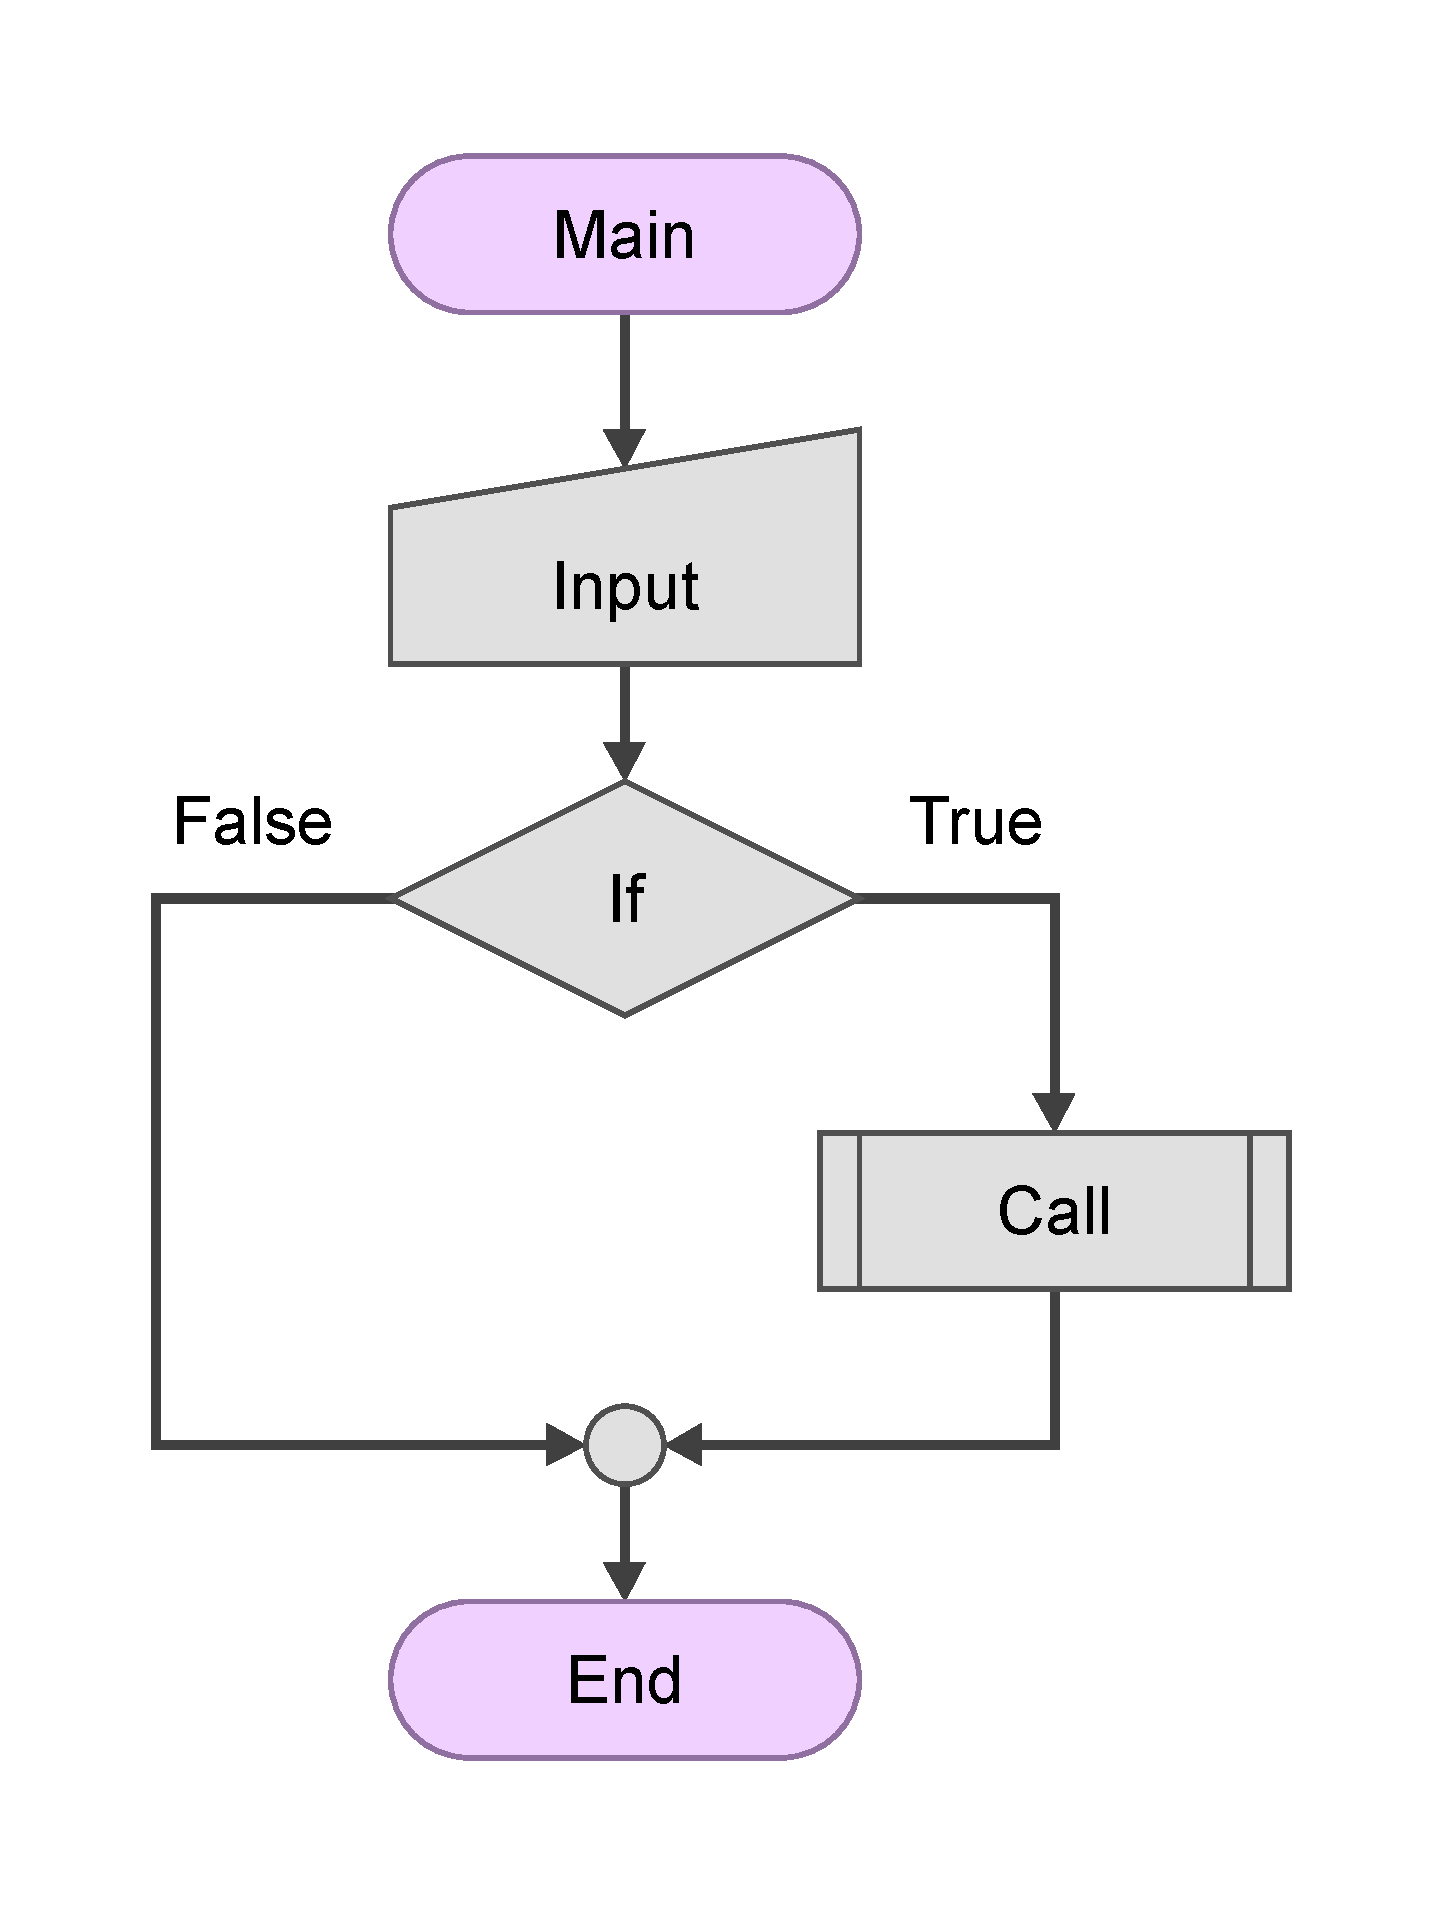
\includegraphics[scale=0.3]{figures/chart.pdf}
  \caption{Example figure in \LaTeX.}
  \label{fig:chart_a}
\end{figure}

\clearpage %  use command \clearpage when you want section or text to
% appear in the next page.

\section{Example of an algorithm in \LaTeX}
Algorithm~\ref{algo:algo_example} is a good example of an algorithm in \LaTeX.
\begin{algorithm}
  \caption{Example caption: sum of all even numbers}
  \label{algo:algo_example}
  \begin{algorithmic}[1]
    \Require{$ \mathbf{x}  = x_1, x_2, \ldots, x_N$}
    \Ensure{$EvenSum$ (Sum of even numbers in $ \mathbf{x} $)}
    \Statex
    \Function{EvenSummation}{$\mathbf{x}$}
    \State {$EvenSum$ $\gets$ {$0$}}
    \State {$N$ $\gets$ {$length(\mathbf{x})$}}
    \For{$i \gets 1$ to $N$}
    \If{$ x_i\mod 2 == 0$}  \Comment Check whether a number is even.
    \State {$EvenSum$ $\gets$ {$EvenSum + x_i$}}
    \EndIf
    \EndFor
    \State \Return {$EvenSum$}
    \EndFunction
  \end{algorithmic}
\end{algorithm}

\section{Example of code snippet  in \LaTeX}

Code Listing~\ref{list:python_code_ex} is a good example of including
a code snippet in a report. While using code snippets, take care of
the following:
\begin{itemize}
  \item do not paste your entire code (implementation) or everything
    you have coded. Add code snippets only.
  \item The algorithm shown in Algorithm~\ref{algo:algo_example} is
    usually preferred over code snippets in a technical/scientific report.
  \item Make sure the entire code snippet or algorithm stays on a
    single page and does not overflow to another page(s).
\end{itemize}

Here are three examples of code snippets for three different
languages (Python, Java, and CPP) illustrated in
Listings~\ref{list:python_code_ex}, \ref{list:java_code_ex}, and
\ref{list:cpp_code_ex} respectively.

\begin{lstlisting}[language=Python, caption={Code snippet in \LaTeX ~and  this is a Python code example}, label=list:python_code_ex]
import numpy as np

x  = [0, 1, 2, 3, 4, 5] # assign values to an array
evenSum = evenSummation(x) # call a function

def evenSummation(x):
    evenSum = 0
    n = len(x)
    for i in range(n):
        if np.mod(x[i],2) == 0: # check if a number is even?
            evenSum = evenSum + x[i]
    return evenSum
\end{lstlisting}

Here we used  the ``\textbackslash clearpage'' command and forced-out
the second listing example onto the next page.
\clearpage  %
\begin{lstlisting}[language=Java, caption={Code snippet in \LaTeX ~and  this is a Java code example}, label=list:java_code_ex]
public class EvenSum{
    public static int evenSummation(int[] x){
        int evenSum = 0;
        int n = x.length;
        for(int i = 0; i < n; i++){
            if(x[i]%2 == 0){ // check if a number is even?
                evenSum = evenSum + x[i];
            }
        }
        return evenSum;
    }
    public static void main(String[] args){
        int[] x  = {0, 1, 2, 3, 4, 5}; // assign values to an array
        int evenSum = evenSummation(x);
        System.out.println(evenSum);
    }
}
\end{lstlisting}

\begin{lstlisting}[language=C, caption={Code snippet in \LaTeX ~and  this is a C/C++ code example}, label=list:cpp_code_ex]
int evenSummation(int x[]){
    int evenSum = 0;
    int n = sizeof(x);
    for(int i = 0; i < n; i++){
        if(x[i]%2 == 0){ // check if a number is even?
            evenSum = evenSum + x[i];
      }
    }
    return evenSum;
}

int main(){
    int x[]  = {0, 1, 2, 3, 4, 5}; // assign values to an array
    int evenSum = evenSummation(x);
    cout<<evenSum;
    return 0;
}
\end{lstlisting}

\section{Example of in-text citation style}
\subsection{Example of the equations and illustrations placement and
reference in the text}
Make sure whenever you refer to the equations, tables, figures,
algorithms,  and listings for the first time, they also appear
(placed) somewhere on the same page or in the following page(s).
Always make sure to refer to the equations, tables and figures used
in the report. Do not leave them without an \textbf{in-text
citation}. You can refer to equations, tables and figures more them once.

\subsection{Example of the equations and illustrations style}
Write \textbf{Eq.} with an uppercase ``Eq`` for an equation before
using an equation number with (\textbackslash eqref\{.\}). Use
``Table'' to refer to a table, ``Figure'' to refer to a figure,
``Algorithm'' to refer to an algorithm and ``Listing'' to refer to
listings (code snippets). Note that, we do not use the articles
``a,'' ``an,'' and ``the'' before the words Eq., Figure, Table, and
Listing, but you may use an article for referring the words figure,
table, etc. in general.

For example, the sentence ``A report structure is shown in
\textbf{the} Table~\ref{tab:gen_template}'' should be written as ``A
report structure is shown \textbf{in} Table~\ref{tab:gen_template}.''

\section{Summary}
Write a summary of this chapter.

~\\[5em]
\noindent
{\huge\textbf{Note:}} In the case of \textbf{software engineering}
project a Chapter ``\textbf{Testing and Validation}'' should precede
the ``Results'' chapter. See Section~\ref{subsec:se_chpters} for
report organization of such project.

\chapter{Conclusions and Future Work}
\label{ch:con}
\section{Conclusions}
Typically a conclusions chapter first summarizes the investigated problem and its aims and objectives. It summaries the critical/significant/major findings/results about the aims and objectives that have been obtained by applying the key methods/implementations/experiment set-ups. A conclusions chapter draws a picture/outline of your project's central and the most signification contributions and achievements. 

A good conclusions summary could be approximately 300--500 words long, but this is just a recommendation.

A conclusions chapter followed by an abstract is the last things you write in your project report.

\section{Future work}
This section should refer to Chapter~\ref{ch:results} where the author has reflected their criticality about their own solution. Concepts for future work are then sensibly proposed in this section.

\textbf{Guidance on writing future work:} While working on a project, you gain experience and learn the potential of your project and its future works. Discuss the future work of the project in technical terms. This has to be based on what has not been yet achieved in comparison to what you had initially planned and what you have learned from the project. Describe to a reader what future work(s) can be started from the things you have completed. This includes identifying what has not been achieved and what could be achieved. 



A good future work summary could be approximately 300--500 words long, but this is just a recommendation.
\chapter{Reflection}
\label{ch:reflection}
%%%%%%%%%%%%%%%%%%%%%%%%%%%%%%%
%% Please remove/replace text below
%%%%%%%%%%%%%%%%%%%%%%%%%%%%%%%
Write a short paragraph on the substantial learning experience. This can include your decision-making approach in problem-solving.

\textbf{Some hints:} You obviously learned how to use different programming languages, write reports in \LaTeX and use other technical tools. In this section, we are more interested in what you thought about the experience. Take some time to think and reflect on your individual project as an experience, rather than just a list of technical skills and knowledge. You may describe things you have learned from the research approach and strategy, the process of identifying and solving a problem, the process research inquiry, and the understanding of the impact of the project on your learning experience and future work.

Also think in terms of:
\begin{itemize}
    \item what knowledge and skills you have developed
    \item what challenges you faced, but was not able to overcome
    \item what you could do this project differently if the same or similar problem would come
    \item rationalize the divisions from your initial planed aims and objectives.
\end{itemize}


A good reflective summary could be approximately 300--500 words long, but this is just a recommendation.

~\\[2em]
\noindent
{\huge \textbf{Note:}} The next chapter is ``\textbf{References},'' which will be automatically generated if you are using BibTeX referencing method. This template uses BibTeX referencing.  Also, note that there is difference between ``References'' and ``Bibliography.'' The list of ``References'' strictly only contain the list of articles, paper, and content you have cited (i.e., refereed) in the report. Whereas Bibliography is a list that contains the list of articles, paper, and content you have cited in the report plus the list of articles, paper, and content you have read in order to gain knowledge from. We recommend to use only the list of ``References.'' 


% -------------------------------------------------------------------
% Bibliography/References  -  Harvard Style was used in this report
% -------------------------------------------------------------------
\bibliography{references}  %  Patashnik, O. (1988), BibTEXing.
% Documentation for general BibTEX users.

% -------------------------------------------------------------------
% Appendices
% -------------------------------------------------------------------

\begin{appendices}
  \chapter{An Appendix Chapter (Optional)}
\label{appn:A}
% Optional chapter
Some lengthy tables, codes, raw data, length proofs, etc. which are \textbf{very important but not essential part} of the project report goes into an Appendix. An appendix is something a reader would consult if he/she needs extra information and a more comprehensive understating of the report. Also, note that you should use one appendix for one idea.

An appendix is optional. If you feel you do not need to include an appendix in your report, avoid including it. Sometime including irrelevant and unnecessary materials in the Appendices may unreasonably increase the total number of pages in your report and distract the reader.


\end{appendices}

\end{document}
